\documentclass{beamer}

\usefonttheme[onlymath]{serif}
\usepackage[utf8]{inputenc}
\usepackage{amsmath}
\usepackage{array}
\usepackage{graphicx}
\usepackage{mathtools}
\usepackage{minted}
\usepackage{hyperref}
\hypersetup{
    colorlinks=true,
    linkcolor=blue,
}
\usemintedstyle{manni}
\newminted{python}{fontsize=\footnotesize}
\newminted{cython}{fontsize=\footnotesize}

\usetheme{Pittsburgh}
% \beamertemplatenavigationsymbolsempty

\usepackage{tikz,tkz-euclide}
\usetikzlibrary{angles}
\usetikzlibrary{decorations.markings}
\tikzset{%
  ->-/.style={decoration={markings, mark=at position 0.5 with {\arrow{>}}},
              postaction={decorate}},
  ->>-/.style={decoration={markings, mark=at position 0.5 with {\arrow{>>}}},
               postaction={decorate}},
  -|-/.style={decoration={markings, mark=at position 0.5 with {|}},
              postaction={decorate}},
}

\usepackage{pgfpages}
\setbeamertemplate{note page}{\pagecolor{yellow!5}\insertnote}
\setbeameroption{show notes on second screen=right}

\DeclareMathOperator{\md}{Manhattan Distance}

\title{Crunching Numbers with NumPy and Cython}
\author{Brian Lester}
\institute{interactions}
\date{\today}

\begin{document}

\def\R{\mathbb{R}}
\frame{\titlepage}

\begin{section}{Bio}

\begin{frame}
    \frametitle{Me}
    \begin{itemize}
        \item Work on NLP at Interactions specializing in Deep Learning
        \item Published/Maintain several python packages
        \begin{itemize}
            \item \href{https://github.com/blester125/string-distance}{string-distance}
            \item \href{https://github.com/blester125/text-rank}{text-rank}
            \item \href{https://github.com/dpressel/mead-baseline}{mead-baseline}
        \end{itemize}
    \end{itemize}
    \note{
        \begin{itemize}
            \item We use chat bots to ``facilitate customer care interaction'' aka to build better chat bots
            \item I mostly do DL and am a big Nerd so if you every want to talk about ML for NLP I'm game
            \item Python is my daily driver
            \item Have several packages on PyPI including ones written in cython, the subject of today's talk
        \end{itemize}
    }
\end{frame}

\end{section}

\begin{section}{Background}

\begin{frame}
    \frametitle{The Problem}
    \begin{center}
    \begin{figure}
        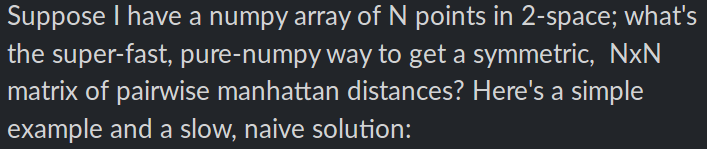
\includegraphics[width=\linewidth]{images/problem.png}
        \caption{\href{https://a2mads.herokuapp.com/}{Ann Arbor Machine Learning and Data Science Slack}}
    \end{figure}
    \end{center}
    \note{
        \begin{itemize}
            \item Ann Arbor Machine Learning and Data Science Slack we call it a2mads
            \item There aren't a lot of messages flying about but when someone asks a question there is normally a lot if discussion
            \item This user was asking that given a list of points what is the distance between this point and every other point in the list
            \item There was a long thread about how to optimize his solution, we will walk through some of them.
        \end{itemize}
    }
\end{frame}

\begin{subsection}{Manhattan Distance}

\begin{frame}<1>[label=md]
    \frametitle{Manhattan Distance}
    \begin{itemize}
        \item<1-> The distance between points measured along axes at right angles
        \item<2-> Also called the L1, cityblock, or taxi distance
    \end{itemize}
    \note{
        \begin{itemize}
            \item Distance if you can only move along the axes
            \item Like you have directions to somewhere in manhattan, you can't walk through a building, you need to walk along the streets
        \end{itemize}
    }
\end{frame}

\begin{frame}[label=block]
    \begin{center}
        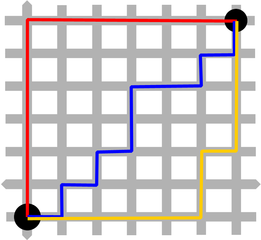
\includegraphics[width=0.9\textwidth]{images/manhattan.png}
    \end{center}
\end{frame}

\againframe<2->{md}

\begin{frame}
    \frametitle{Manhattan Distance}
        A point in $M$ dimensions is a vector of $M$ integers where the values at index $i$ is the distance along the $i^{th}$ axis.
\end{frame}

\begin{frame}
    \frametitle{Manhattan Distance}
        \begin{align*}
            X &\in \R^{M} \\
            Y &\in \R^{M} \\
            \md(X, Y) &= \sum_i^M | X_i - Y_i |
        \end{align*}
\end{frame}

\againframe{block}

\begin{frame}
    \frametitle{Proof of Equal Lengths}
    \begin{columns}
        \column{0.5\textwidth}
          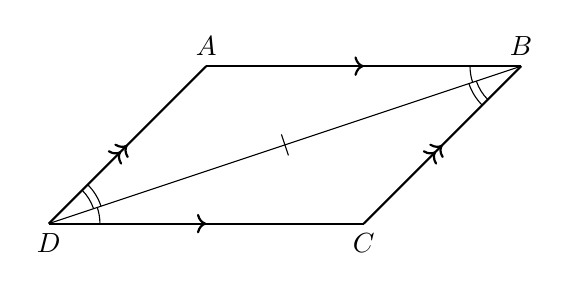
\begin{tikzpicture}[xslant=1,xscale=2,scale=2]
              \coordinate (D) at (0,0);
              \coordinate (A) at (0,1);
              \coordinate (B) at (1,1);
              \coordinate (C) at (1,0);
              \draw[-,thick,->-] (A) node[above]{$A$} -- (B) node[above]{$B$};
              \draw[-,thick,->-] (D) node[below]{$D$} -- (C) node[below]{$C$};
              \draw[-,thick,->>-] (D) -- (A);
              \draw[-,thick,->>-] (C) -- (B);
              \draw[-] (D) -- (B);
              \tkzMarkSegment[mark=|](D,B)
              \draw pic[draw=black,-,angle eccentricity=1.2,angle radius=0.6cm] {angle=B--D--A};
              \draw pic[draw=black,-,angle eccentricity=1.2,angle radius=0.7cm] {angle=B--D--A};
              \draw pic[draw=black,-,angle eccentricity=1.2,angle radius=0.6cm] {angle=D--B--C};
              \draw pic[draw=black,-,angle eccentricity=1.2,angle radius=0.7cm] {angle=D--B--C};
              \draw pic[draw=black,-,angle eccentricity=1.2,angle radius=0.65cm] {angle=A--B--D};
              \draw pic[draw=black,-,angle eccentricity=1.2,angle radius=0.65cm] {angle=C--D--B};
          \end{tikzpicture}
        \column{0.5\textwidth}
            \begin{align}
                \overline{AB} &\parallel \overline{DC} \\
                \overline{AD} &\parallel \overline{BC} \\
                \angle ABD &\cong \angle CDB \\
                \angle ADB &\cong \angle DBC \\
                \overline{DB} &= \overline{DB} \\
                \triangle ADB &\cong \triangle{CDB} \\
                \overline{AB} &= \overline{CD} \\
                \overline{AD} &= \overline{CB}
            \end{align}
    \end{columns}
    \note{
        \begin{enumerate}
            \item AB and DC are parallel by the definition of a parallelogram
            \item AD and BC are parallel by the definition of a parallelogram
                \begin{itemize}
                    \item  DB is a transversal of both sets of parallel lines
                \end{itemize}
            \item ABD and CDB are congruent because they are alternate interior angles
            \item ADB and DBC are congruent because they are alternate interior angles
            \item It is the same length as itself
            \item Triangles are congruent by angle side angle
            \item AB and CD are the same because they are the same sides of congruent triangles
            \item AD and CB are the same because they are the same sides of congruent triangles
        \end{enumerate}
    }
\end{frame}

\begin{frame}
    \frametitle{Proof of Shortest Path}
\end{frame}

\end{subsection}

\begin{frame}
    \frametitle{NumPy}
    \begin{itemize}
        \item<1-> \href{https://docs.scipy.org/doc/numpy/reference/}{NumPy}: A collection of linear algebra functions that operate on a \tt{ndarray}
        \item<2-> \tt{ndarray} is a type container that can represent multi-dimensional arrays
        \item<3-> The majority of functionality is implemented in C extensions for speed
    \end{itemize}
    \note{
        \begin{itemize}
            \item \tt{ndarray} has a data type
            \begin{itemize}
                \item all the items in it need to be the same and they can be stored contiguously in memory.
                \item So instead of following pointers for to the object for each element in a python list we can access the element directly
                \item This makes access fast and because they are together in memory we get better cache utilization
            \end{itemize}
            \item \tt{ndarray} is a multi dimensional array
            \begin{itemize}
                \item a thing is a scalar
                \item a list of things is an array (or vector)
                \item a list of arrays is a matrix
                \item a list of matrices is a \tt{ndarray}
                \item You can index like \tt{x[i, j, k]}
                \item can have an arbitrary dimensions
            \end{itemize}
            \item A C extension is code writen in C that can be called from python. You can use the speed of C and let go of the GIL. Loses ease of Python
        \end{itemize}
    }
\end{frame}

\begin{frame}
    \frametitle{Cython}
    \begin{itemize}
        \item<1-> \href{https://cython.org/}{Cython} is a compiler for Python and Cython
        \item<2-> It creates C extensions
        \item<3-> It looks more like python than C, but adds types
        \item<4-> You can call python code from inside the C extension
        \item<5-> It can compile pure python code
        \item<6-> Makes it easy to wrap C libraries
    \end{itemize}
    \note{
        \begin{itemize}
            \item Cython is a superset of python, adds things like static types
            \item Compiling just python gives a slight speed boost
        \end{itemize}
    }
\end{frame}

\end{section}


\begin{frame}[fragile]
\frametitle{Python v1}

    \begin{pythoncode}
def pairwise_manhattan_python_v1(
    points: List[List[int]]
) -> List[List[int]]:
    results = []
    # For each pair of points
    for i in range(len(points)):
        dist_i_j = []
        for j in range(len(points)):
            # Manhattan distance
            dist_i_j.append(sum(
                abs(p1 - p2) for p1, p2 in zip(points[i], points[j])
            ))
        results.append(dist_i_j)
    return results
    \end{pythoncode}

\end{frame}


\begin{frame}[fragile]
\frametitle{Python v2}

    \begin{pythoncode}
def pairwise_manhattan_python_v2(
    points: List[List[int]]
) -> List[List[int]]:
    # Preallocate the results
    results = [[None] * len(points) for _ in range(len(points))]
    # Look at every pair of you and the ones after you, distances
    # with points before you were calculated when they looked at you
    for i in range(len(points)):
        for j in range(i, len(points)):
            # Manhattan distance calculation
            dist = sum(
                abs(p1 - p2) for p1, p2 in zip(points[i], points[j])
            )
            # Manhattan distance is symmetric
            results[i][j] = dist
            results[j][i] = dist
    return results
    \end{pythoncode}

\end{frame}

\begin{frame}
    \frametitle{Manhattan Distance}
    \begin{align*}
        X &\in \R^{M} \\
        Y &\in \R^{M} \\
        \md(X, Y) &= \sum_i^M | X_i - Y_i |
    \end{align*}
    \note{
        \begin{itemize}
            \item Even though there is a subtraction which isn't commuatitive there is an absoulte value so it doesn't matter which is substracted from whick
        \end{itemize}
    }
\end{frame}

\begin{frame}[fragile]
\frametitle{Numpy v1}

    \begin{pythoncode}
def pairwise_manhattan_numpy_v1(
    points: List[np.ndarray]
) -> np.ndarray:
    results = np.zeros((len(points), len(points)), dtype=np.int32)
    for i in range(len(points)):
        for j in range(len(points)):
            results[i, j] = np.sum(np.abs(points[i] - points[j]))
    return results
    \end{pythoncode}
\end{frame}


\begin{frame}[fragile]
\frametitle{Numpy v2}

    \begin{pythoncode}
def pairwise_manhattan_numpy_v2(
    points: List[np.ndarray]
) -> np.ndarray:
    results = np.zeros((len(points), len(points)), dtype=np.int32)
    for i in range(len(points)):
        for j in range(i, len(points)):
            dist = np.sum(np.abs(points[i] - points[j]))
            results[i, j] = dist
            results[j, i] = dist
    return results
    \end{pythoncode}
\end{frame}

\begin{frame}[fragile]
\frametitle{Numpy v3}

    \begin{pythoncode}
def pairwise_manhattan_numpy_v3(points: np.ndarray) -> np.ndarray:
    results = []
    for i in range(len(points)):
        results.append(np.sum(np.abs(points[i] - points), axis=-1))
    return np.stack(results)

    \end{pythoncode}
\end{frame}

\begin{frame}[fragile]
\frametitle{Numpy v4}

    \begin{pythoncode}
def pairwise_manhattan_numpy_v4(points: np.ndarray) -> np.ndarray:
    exp_points = np.expand_dims(points, 1)  # [N, 1, M]
    return np.sum(np.abs(exp_points - points), axis=-1)
    \end{pythoncode}
\end{frame}

\begin{section}{Manhattan Distance in Cython}

\begin{frame}[fragile]
\frametitle{Cython Implementation}
    \begin{cythoncode}
@cython.wraparound(False)
@cython.boundscheck(False)
cpdef int[:, :] pairwise_manhattan(int[:, :] points):
    cdef int n = points.shape[0]
    cdef int m = points.shape[1]
    results = np.zeros((n, n), dtype=np.int32)
    cdef int[:, :] results_view = results
    cdef int i, j, k, dist
    for i in range(n):
        for j in range(i, n):
            dist = 0
            for k in range(m):
                dist += abs(points[i, k] - points[j, k])
            results_view[i, j] = dist
            results_view[j, i] = dist
    return results

    \end{cythoncode}
\end{frame}

\begin{frame}[fragile]
\frametitle{Cython Decorators}
    \begin{cythoncode}
@cython.wraparound(False)
@cython.boundscheck(False)
    \end{cythoncode}
\end{frame}

\end{section}

\end{document}
